\section{Method}

\paragraph{Backbone.} We use a DGCNN-style graph network with a single shared (static) learned adjacency and
a Chebyshev graph convolution over electrode nodes, exposing
$\texttt{forward\_graph}(x) \rightarrow (\text{logits}, \texttt{graph\_z}, \texttt{node\_z},
\texttt{edge\_logits})$. Because the adjacency is shared across samples, there is \textbf{no per-sample edge
object} ($\texttt{edge\_logits} = \texttt{None}$); CIGL as studied here is therefore \textbf{graph/node only}.
We adopt this backbone after an explicit search (Section~\ref{sec:analysis}): it is the graph-compatible
backbone we found that actually learns the task.

\paragraph{Leakage objects and proxy.} Let $Z_g$ be the graph readout and $Z_v$ the per-electrode node
features, $Y$ the class label, and $D$ the source-domain (subject) label. We quantify label-conditional
domain leakage with a \textbf{posterior-KL plug-in proxy}:
\begin{align}
R_g &= \mathbb{E}\!\left[ \mathrm{KL}\!\left( q_g(D \mid Z_g, Y) \,\Vert\, \pi_y(D) \right) \right], &
R_n &= \frac{1}{C} \sum_{v} \mathbb{E}\!\left[ \mathrm{KL}\!\left( q_n(D \mid Z_v, v, Y) \,\Vert\,
\pi_y(D) \right) \right],
\end{align}
where $q_g$/$q_n$ are conditional-domain posterior heads, $\pi_y(D)$ the within-label domain prior, and $C$
the number of electrodes. We stress that $R_g$/$R_n$ are a \textbf{proxy}, not an unbiased CMI estimator.

\paragraph{Regularizer.} CIGL trains the backbone with $\mathcal{L} = \mathcal{L}_{\mathrm{CE}} +
\lambda_g R_g + \lambda_n R_n$ (no edge term), using the established two-step scheme: Step~A fits the
posterior heads on detached features; Step~B penalizes the encoder. Throughout the confirmation we use a
single \textbf{fixed} weight $\lambda_g = \lambda_n = 0.010$ ($\lambda_{\mathrm{edge}} = 0$). The pipeline is
sketched in Figure~\ref{fig:pipeline}.

% Figure 2 Panel A/B (see paper/cmi_trace/MANUSCRIPT_INTEGRATION.md, P0.3): the study-architecture / audit
% pipeline is split into TWO panels joined by a DASHED bridge -- Panel A = same-backbone objective audit
% (the P0.1/P0.2 contribution; CIGL's static-adjacency DGCNN + posterior-KL is the Encoder-CMI objective in
% this panel), Panel B = complementary representation-level (EEGNet/TSMNet geometry + deployment) extension.
% The objective comparison (P0.1) is still producing (jobs 896396/896397); this figure shows the STUDY
% DESIGN, not results. Schematic only; no result numbers are asserted here.
\begin{figure}[t]
  \centering
  \fbox{\parbox{0.92\linewidth}{\centering\small\textbf{[F2 --- study architecture, schematic, DRAFT]}\\[3pt]
  \textbf{Panel A --- same-backbone objective audit.}\\[1pt]
  ERM / CORAL / C-CORAL / IRMv1 / V-REx / conditional-adversarial / Encoder-CMI
  (\emph{all} on the \textbf{same} static-adjacency DGCNN adapter, source-only LOSO, cloned init; CIGL's
  \texttt{graph\_z}/\texttt{node\_z} posterior-KL, $\lambda=0.010$, is the Encoder-CMI objective)
  $\rightarrow$ marginal $+$ class-conditional moment gaps
  $\rightarrow$ graph/node encoder-CMI $+$ retrained within-label permutation null
  $\rightarrow$ per-domain risk variance $+$ IRMv1 diagnostic (post hoc)
  $\rightarrow$ exact original-head reliance $R_{\mathrm{rel}}(k{=}2)$ $+$ same-rank random control
  $\rightarrow$ target balanced accuracy. \\[4pt]
  $-\;-\;-\;-\;-$\; \emph{dashed bridge: complementary representation-level extension} \;$-\;-\;-\;-\;-$ \\[4pt]
  \textbf{Panel B --- complementary geometry \& deployment extension.}\\[1pt]
  EEGNet / TSMNet frozen representations
  $\rightarrow$ TOS / LEACE / RLACE / INLP / random-$k$
  $\rightarrow$ nonlinear subject residual
  $\rightarrow$ capacity factorial
  $\rightarrow$ source-fitted target deployment. \\[2pt]
  \textit{Draft vector asset: \texttt{figures/fig1\_pipeline\_draft.svg} (to be regenerated as two panels).}}}
  \caption{Study architecture (schematic draft). \textbf{Panel A} is the same-backbone objective audit: every
  objective is trained on the \emph{same} static-adjacency DGCNN adapter under the same source-only LOSO
  protocol and passed through one shared audit; CIGL's graph/node posterior-KL regularizer is the
  Encoder-CMI objective within this panel. \textbf{Panel B}, joined only by a \emph{dashed} bridge, is a
  \emph{complementary representation-level extension} on EEGNet/TSMNet frozen features (geometry probes and
  source-fitted target deployment); it is \textbf{not} claimed that every Panel-A objective underwent every
  TOS / deployment test. The posterior-KL terms are a proxy, not an unbiased CMI estimator.}
  \label{fig:pipeline}
\end{figure}

\paragraph{Audit.} To judge significance we re-fit fresh held-out conditional-domain probes on frozen
features and compare to a \textbf{retrained, within-label permutation null} (permuting $D$ within label on
the probe-training split only, preserving the within-label prior);
$\texttt{clears\_null} = (\texttt{kl\_mean} > \texttt{permutation\_mean})\;\wedge\;
(\texttt{permutation\_p} \le 0.05)$. The audit is the same proxy used as a measurement, never inverted into
an information-theoretic guarantee. Figure~\ref{fig:audit} shows the audit against the null on the
development fold.

\begin{figure}[t]
  \centering
  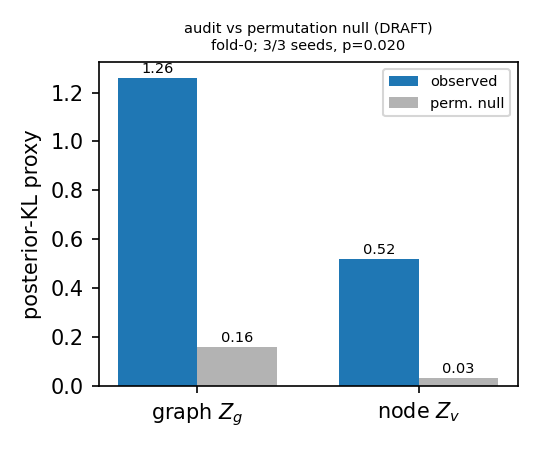
\includegraphics[width=0.5\linewidth]{figures/fig3_audit_null_draft.png}
  \caption{\textbf{[DRAFT, from data]} Source-only leakage audit on BNCI2014\_001 fold-0: observed
  posterior-KL proxy vs the retrained within-label permutation null for the graph and node objects (clears
  the null in 3/3 seeds, $p=0.020$). Values from the development-fold audit; not an unbiased CMI estimate.}
  \label{fig:audit}
\end{figure}

% CMI-Trace P1.5 notation clarification: distinct symbols for the in-loop training regularizer vs the
% held-out audit estimate; "cross-fitted neural posterior plug-in estimate" (no bound proved); raw nats +
% secondary normalized readout; finite-critic underfitting can UNDER-report leakage.
\paragraph{Notation and the training/audit distinction.} We keep the \emph{in-loop training regularizer}
$\mathcal{L}^{\mathrm{CMI}}_{\mathrm{train}} = \lambda_g R_g + \lambda_n R_n$ (computed on the training split
--- on detached features in Step~A and as the encoder penalty in Step~B) notationally distinct from the
\emph{held-out audit estimate} $\hat{I}_{\mathrm{audit}}$, obtained by re-fitting fresh conditional-domain
probes on frozen held-out features. $\hat{I}_{\mathrm{audit}}$ is a \textbf{cross-fitted neural posterior
plug-in estimate}; no information-theoretic bound is proved for it. The two quantities share the posterior-KL
form but are computed on disjoint data and are \emph{not} interchangeable. Because a finite-capacity critic
can \emph{under}-report leakage, $\hat{I}_{\mathrm{audit}}$ is a lower-confidence proxy, never a guarantee. We
report $\hat{I}_{\mathrm{audit}}$ in raw nats, with a secondary normalized readout
$\hat{I}_{\mathrm{audit}} / \hat{H}(D \mid Y)$ used only for cross-dataset comparison.
